
\chapter[A Proposta]{A PROPOSTA}

A proposta deste trabalho é criar uma plataforma, denominada gamifier, de apoio a construção de projetos de gamificação e capaz de exportar projetos para o funifier e importar projetos do funfifier. A plataforma servirá para automatizar o processo de criação dos projetos, simplificar e incentivar a inserção de gamificação no cotidiano das pessoas que tem interesse pelo tema e querem aplicá-lo as suas vidas.

 Este capítulo está estruturado da seguinte maneira: a seção 1 é a introdução, onde será feita uma contextualização sobre o porque de se construir o gamifier com tal propósito e a seção 2, construção da plataforma, onde é descrito o processo de construção da ferramenta.           

\section{Introdução}

 

Segundo \cite{chou2015actionable} gamificação é o ato de cuidadosamente aplicar ao mundo real e as atividades produtivas e os elementos divertidos e envolventes dos jogos. O que torna o ato de gamificar mais complexo que apenas incorporar elementos de jogos em outros contextos. Gamificar é mais sobre  motivar pessoas e menos sobre pontos e troféus \cite{chou2015actionable}, \cite{zichermann2011gamification}. A gamificação é um tema que diz respeito ao ser humano. Gamificação é um novo olhar sobre motivação, vai além de inserir elementos de jogos em contextos fora de jogos, gamificar é trazer pra vida real o incentivo natural que se tem ao jogar jogar um jogo.  É tentar despertar em atividades do cotidiano a mesma sensação que se tem ao jogar.

Ninguém tem que jogar um jogo, as pessoas tem que trabalhar e pagar sua contas, elas não são obrigadas a jogar, mas jogam \cite{chou2015actionable},  \cite{mcgonigal2011reality} e se sentem motivadas, felizes e incentivadas a dar o melhor de si quando estão jogando. Porque as pessoas se sentem motivadas a jogar mas não sentem a mesma motivação na vida real, para conquistar objetivos? O que falta? Motivação? Disciplina? Um modelo de incentivo que funcione? O jogo gera mais esperança de sucesso nas pessoas, em comparação ao jogos, a realidade não demonstra esperança \cite{mcgonigal2011reality}.

As pessoas têm tanto interesse em jogar e não dispõem do mesmo interesse para realizar ou concluir tarefas cotidianas ou conquistar uma meta a longo prazo. É possível deixar esses aspectos da vida mais divertidos e motivadores, jogos podem mudar vidas e motivar pessoas, então a gamificação também pode.

Porque não construir uma plataforma que dê suporte as oportunidades de aplicar a vida real a motivação intrinsecamente ligada aos jogos? Uma ferramenta capaz de dispensar do usuário o conhecimento prévio que ele precisaria ter para construir um projeto de gamficação com chances de dar certo? Um sistema que motive as pessoas a mudar algo fazendo uso de gamificação, pode ser a forma de lecionar uma aula, um percurso utilizado em um tratamento de reabilitação motora, pode ser o hábito da falta de estudo diário, muita coisa pode ser fruto de um projeto de gamificação.

Há algumas décadas têm-se estudado a motivação intrinsecamente ligada ao jogo e como aplicá-la em outras áreas com o mesmo sucesso. Motivar apenas não basta, motivação acaba, é preciso pensar maneiras de manter a motivação, criar um ciclo onde além de motivadas as pessoas permaneçam disciplinadas, não por obrigação, e sim porque sentem vontade de sempre seguir adiante. 

A proposta de criar uma plataforma que apoie a criação de projetos motivadores do início ao fim e o auxiliem as pessoas a conquistar uma meta de maneira disciplinada e divertida e apenas por  obrigação. Uma plataforma que consiga agregar os pontos positivos da gamificação e aplicá-los a vida real.

A ferramenta existirá para que o nivel de conhecimento exigido atualmente para se criar um projeto de gamificação seja diminuído. O usuário não vai precisar estudar gamificação para conseguir montar um projeto de gamificação, ela fará isso de maneira guiada e intuitiva.

Pretende-se também que com o uso do gamifier, o usuário com algum grau de conhecimento relacionado ao assunto tenha sua produtividade elevada no momento da construção do projeto. Para que o sistema resulte em bons projetos ele será constituído de elementos que darão suporte a uma gamificação coerente.

\section{Construção do Gamifier}

A figura (\ref{fig01}) representa os componentes internos que serão utilizados para dar forma ao gamifier, cada cubo da figura representa as unidades principais, técnicas de gamificação e os atributos das técnicas de gamificação. 

Os cores drives, representados como a parte superior do cubo, são as unidades principais do framework e serão também o principal componente da ferramenta, as técnicas de gamificação, representadas como o lado esquerdo do cubo, compõem as unidades principais, os atributos, representados como o lado direito do cubo, compõem as técnicas de gamificação. 

A plataforma tem como propósito o apoio a construção de projetos gamificação que motivem os seus usuários e ela terá o usuário como foco principal, como indicado na figura, o design focado no ser humano \cite{chou2015actionable} ou design centrado no usuário \cite{kumar2013gamification}, indica que o processo de concepção e desenvolvimento da gamificação será focado no usuário e nas suas motivações. 


\begin{figure}[h]
	\centering
		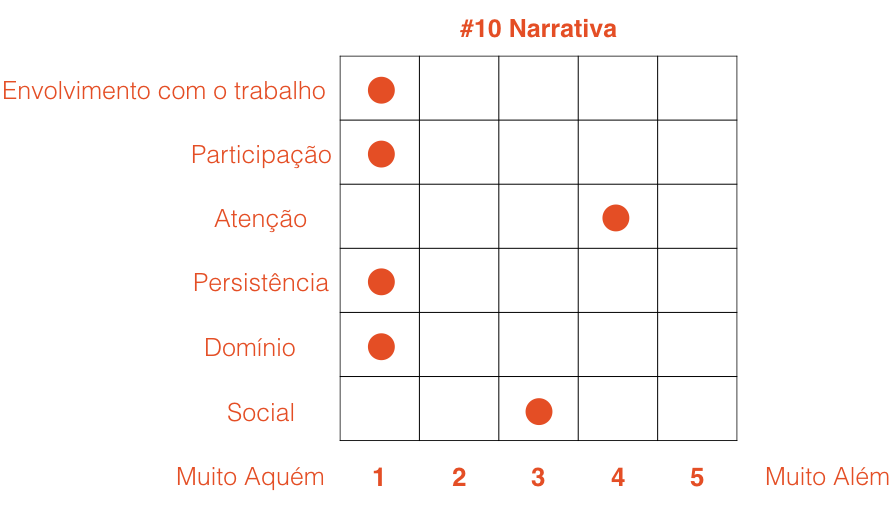
\includegraphics[keepaspectratio=true,scale=0.5]{figuras/notas.png}
	\caption{Composição da Ferramenta.\label{fig01}}
\end{figure}

Para que o gamifier possa ser construído de maneira adequada e que proporcione ao usuário uma experiência bem sucedida na criação do seu projeto, o framework octalysis foi escolhido como alicerce para a construção da ferramenta.

As unidades principais do framework juntamente com as técnicas de gamificação existentes estão bem alinhadas com o principal próposito da ferramenta. 
Chou utiliza as unidades principais do framework para motivar os usuários e as técnicas de gamificação para representar elementos de jogos. As técnicas possuem mais de uma função, são utilizadas também para intensificar a motivação representada pela unidade principal da qual fazem parte. O emprego correto das mesmas na construção do projeto produz um resultado mais satisfatório. Como gamificação é o ato de aplicar elementos de jogos em contexto fora de jogo, as técnicas de gamificação representam a ligação entre o contexto de não jogo ao contexto de jogo. Para que o gamifier produza um bom resultado, as técnicas de gamificação devem ser utilizadas de maneira a se complementarem.

As oito unidades principais do octalysis possuem uma descrição e são compostas por inúmeras técnicas de gamificação, já as técnicas de gamificação possuem uma descrição, mas não é especificado qual a sua composição.  Para construir o gamifier definiu-se então um conjunto de atributos irão compor as técnicas e foi realizado um mapeamento que indicará se há relacionamento entre as técnicas e como isso influencia na construção do projeto de gamificação.

Atualmente não há uma definição formal de um conjunto mínimo de atributos que devem estar presentes para que uma técnica seja implementada corretamente e não havia um mapeamento que informasse ao construtor do projeto de gamificação como as técnicas se relacionam, se é possível implementar todas de uma vez, se a implementação de uma afeta a implementação de outra. Não há uma definição de como deve ser o relacionamento entre as técnicas de gamificação. Isso acarreta uma dificuldade para identificar se o projeto está sendo construído corretamente. Não há também como identificar se uma técnica de gamificação está ligada a mais de uma unidade principal. 

Afim obter a relação das técnicas entre si e das técnicas entre as unidades principais foi realizado o mapeamento das técnicas de gamificação. Inicialmente levantou-se as UPs e as técnicas de gamificação pertencentes as unidades, porém, a primeira fonte de informação não continha todas as técnicas de gamificação presente no octalysis. A busca foi extendida a outros meios.

Como a informação sobre o framework não se encontra centrada em um só lugar. Cada técnica é composta por um identificador representado por uma \#, seguido de um número, \#10 narrativa, por exemplo, e uma descrição, para facilitar o entendimento da técnica, atualmente além das oito unidades principais foram mapeadas 43 técnicas de gamificação, mas o relacionamento entre elas ainda não foi definido.

As técnicas de gamificação tem uma descrição simples e intuitiva. É fácil entender o que a técnica faz e o que ela pretende motivar no usuário.É conhecimento muito atrelado a experiência pessoal de quem propôs a existência e o uso da técnica, quando se faz necessário realizar a implementação, tirar do campo das idéias e colocar em prática, esse conhecimento teórico não é suficiente, porque está muito ligado ao conhecimento adquirido ao longo dos anos pelo especialista em gamificação.

 A proposta aqui é justamente tornar a gamificação acessível também a não especialistas. Para tornar a implementação das técnicas mais tangível, foi definido um conjunto de atributos caracterizadores, que tornam as técnicas de gamificação passíveis de implementação sem que elas percam a identidade ou o foco principal pertencentes a elas. 

 O conjunto de atributos definidos para compor a estrutura interna das técnicas são alguns dos indicadores de engajamento definidos por \cite{fredericks2004school}, os autores dividem, como mencionado no capítulo 2, os engajamentos em três tipos, o engajamento emocional, que trata, por exemplo, de emoções como alegria, interesse e raiva, o engajamento comportamental, que trata de indicadores de conduta, tais como, esforço, atenção e persistência e o engajamento cognitivo, que trata, por exemplo, de flexibilidade para resolver um problema, concentração e domínio.

 Engajamento também pode ser interpretado neste contexto como envolvimento, cada tipo de engajamento possui alguns indicadores, os indicadores caracterizam os tipos de engajamento e foram escolhidos aqui também para caracterizar as técnicas de gamificação, tal como se fossem adjetivos caracterizando as técnicas de gamificação. A estrutura interna das técnicas é igual, independente da técnica de gamificação em questão e foi pautada em aspectos educacionais, outros aspectos não foram levados em consideração para o TCC1 . Os indicadores escolhidos para compor a estrutura interna das técnicas são: 


\begin{itemize}
\item  \textbf {Envolvimento com o trabalho:}  Mensura a quantidade de envolvimento com a gamificação que a técnica exigirá do usuário.
\item  \textbf {Participação:}  Mensura quanta participação efetiva na gamificação a técnica exigirá do usuário
\item  \textbf {Atenção:}  Mensura quanta atenção a gamificação exigirá do usuário.
\item  \textbf {Persistência:} Mensura quão persistente o usuário será para obter resultados no projeto de gamificação. 
\item  \textbf {Domínio:} Mensura a quantidade de maestria que o usuário precisará dispor para executar a técnica de gamificação. 
\item  \textbf{Social:} Mensura a quantidade de envolvimento social que a técnica dispõe para o usuário e quão social a técnica pode ser.
\end{itemize}


Cada indicador representará um atributo da técnica de gamificação e receberá uma valor que representa o grau de pertinência à técnica de gamificação, os valores variam de um a cinco e serão concedidos de acordo com a escala de Likert. A escala de Likert utilizada possui cinco itens: 

\begin{itemize}
\item  \textbf {Nota 1 - Muito aquém:} O atributo influência fracamente a técnica de gamificação
\item  \textbf {Nota 2 - Aquém:} O atributo influencia aquém do normal a técnica de gamificação
\item  \textbf {Nota 3 - Suficiente / Normal:} O atributo influencia de forma suficiente (normal) a técnica de gamificação
\item  \textbf {Nota 4 - Além:} O atributo influência além da normal a técnica de gamificação
\item  \textbf {Nota 5 - Muito além:} O atributo influencia plenamente a técnica de gamificação
\end{itemize}

\newpage


A figura (\ref{fig02}) é um exemplo de pontuação de atributos para a técnica número 10, a narrativa, cada coluna representa uma das notas da escala, a figura conta com a menor nota e a maior nota como exemplo nas extremidades da tabela, a técnica representada na tabela 

\begin{figure}[h]
	\centering
		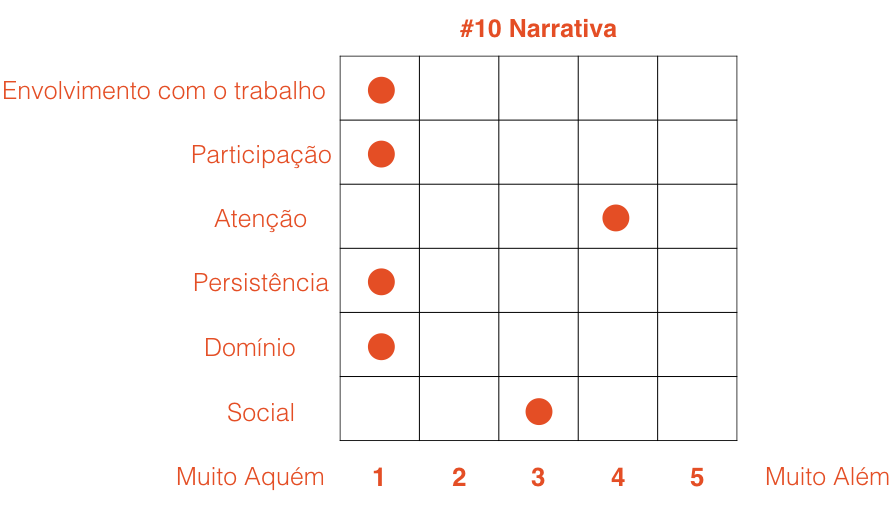
\includegraphics[keepaspectratio=true,scale=0.5]{figuras/notas.png}
	\caption{Representação dos atributos pontuados\label{fig02}}
\end{figure}




A figura (\ref{fig03}) representa a composição da estrutura da ferramenta. Cada unidade principal é composta pelas suas técnicas de gamificação, a unidade principal utilizada como exemplo é a significado épico e chamado, a figura apresenta algumas das técnicas de gamificação pertecentes a esta unidade, como \#10 narrativa, \#23 sorte de iniciante, \#26 elitismo e \#27 herói da humanidade. Cada técnica é composta por seis atributos e cada atributo recebe uma nota de um a cinco. Os atributos têm duas funções, caracterizar as técnicas de gamificação e espelhar o envolvimento do usuário com a gamificação, por exemplo, se a técnica exige do usuário muita atenção e persistência a gamificação também exigirá. Com a definição dos atributos formadores das técnicas é possível visualizar a estrutura interna da ferramenta em si. A ferramenta será composta da unidades principais do octalysis, das técnicas de gamificação e dos atributos das técnicas, os indicadores de engajamento. 


\begin{figure}[h]
	\centering
		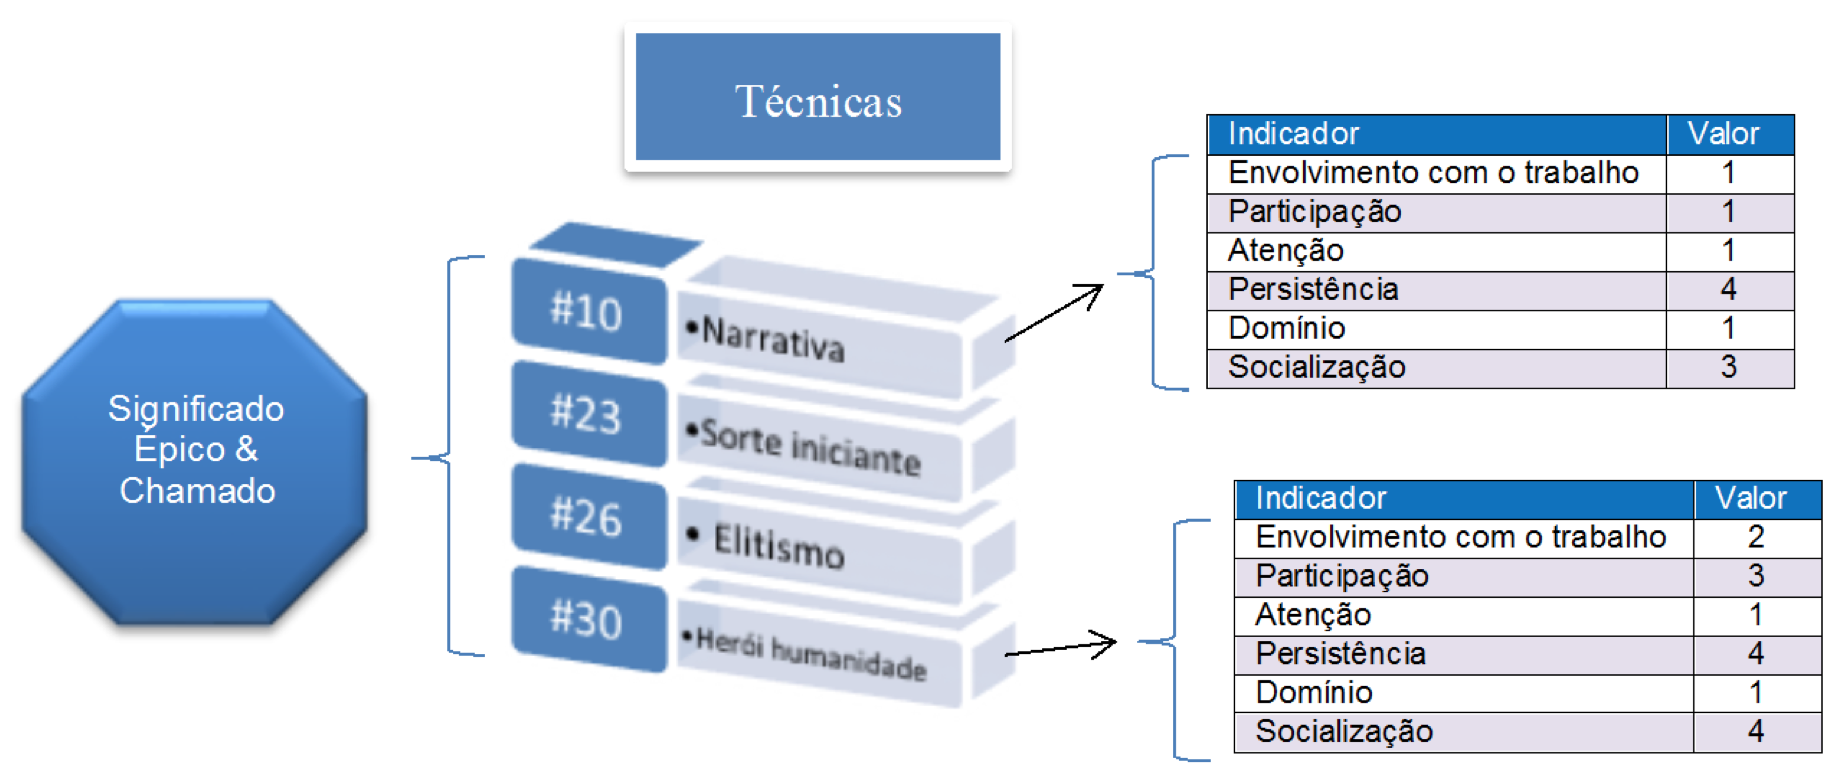
\includegraphics[keepaspectratio=true,scale=0.5]{figuras/mapeamento.eps}
	\caption{Estrutura geral da ferramenta.\label{fig03}
}
\end{figure}
\newpage


Após ser feito o mapeamento de todas as técnicas de gamificação existentes no framework é necessário mapear a ligação entre as mesmas, como mapeamento das técnicas já foi realizado e todos os indicadores receberam os valores pertinentes, o próximo passo é identificar se existe ligação entre as técnicas e se a implementação de uma pode exercer influência positiva ou negativa sobre outra, influenciando a construção do projeto de gamificação que o usuário esteja realizando e se elas podem pertencer a mais de uma unidade principal, infere-se que o mapeamento do relacionamento entre as técnicas irá gerar um grafo. O mapeamento inicial gerou uma estrutura similar a Fig (\ref{fig04}).

\begin{figure}[h]
	\centering
		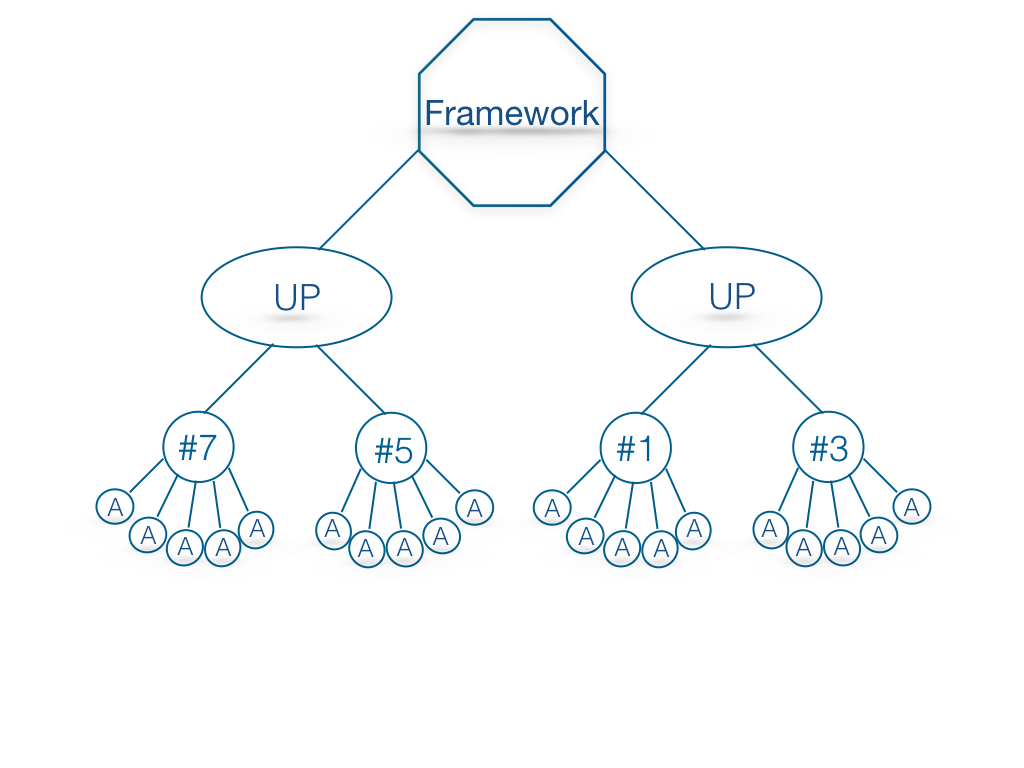
\includegraphics[keepaspectratio=true,scale=0.5]{figuras/heranca.png}
	\caption{Hieraquia dos elementos da ferramenta.	\label{fig04}}
\end{figure}

\newpage

A figura (\ref{fig04}) representa o relacionamento proposto entre as unidades principais, representadas na figura como UP, as técnicas de gamificação, \#número e os atributos das técnicas de gamificação, A. Os componentes estão distribuídos de forma hierárquica, mas a abordagem não necessáriamente seguirá essa restrição, o usuário poderá escolher a forma como irá montar o projeto, o projeto poderá ser iniciado pelas unidades principais, mas a ferramenta também irá dispor da opção de iniciar o projeto pelas técnicas de gamificação e as inter-relações entre as técnicas de gamificação não são necessariamente hierárquicas.

A figura (\ref{fig05}) representa o relacionamento entre as técnicas de gamificação, esse inter-relacionamento também ocorrerá entre as unidades principais, se a técnica de gamificação que pertece a uma determinada unidade principal interage diretamente com uma técnica pertecente a outra unidade, as unidades acabam formando uma relação indireta. 

A figura (\ref{fig05}) demonstra como funcionará o relacionamento entre as técnicas e entre as unidades principais. Como as técnicas possuem o mesmo conjunto de atributos, quando atributos de diferentes técnicas possuem valores parecidos, infere-se que eles despertam no usuário da gamificação as mesmas motivações ou níveis muito próximos de motivação, apesar de serem técnicas diferentes, dessa maneira se dará a construção do relacionamento entre as mesmas, nem todas as técnicas se relacionam e nem todas que se relacionam fazem isso da mesma maneira, nem com a mesma intensidade.

A figura (\ref{fig05}) representa como se dará a o relacionamento entre as técnicas e as unidades principais, \#1UP e \#2UP são as unidades principais e os números seguidos de \# são as técnicas de gamificacão e as linhas representam o relacionamento entre os elementos. Apesar de não estarem presentes visualmente, os atributos também fazem parte deste relacionamento. Como indica a figura, o relacionamento entre as técnicas forma um grafo, onde as técnicas de gamificação e as unidades principais são os vértices e as arestas a ligação entre estes elementos. Quando uma unidade principal está ligada a uma técnica que está ligada a outra unidade principal existe uma relação indireta entre as unidades principais, essa ligação, por exemplo, é representada na figura como relacionamento indireto entre a \#1UP, técnica \#23 e \#2UP. E este relacionamento é que será responsável por indicar a consistência do projeto, como o relacionamento está mapeado internamente, quando o usuário criar um projeto que não está consistente com o relacionamento das técnicas e unidades principais ele será informado.

\begin{figure}[h]
	\centering
		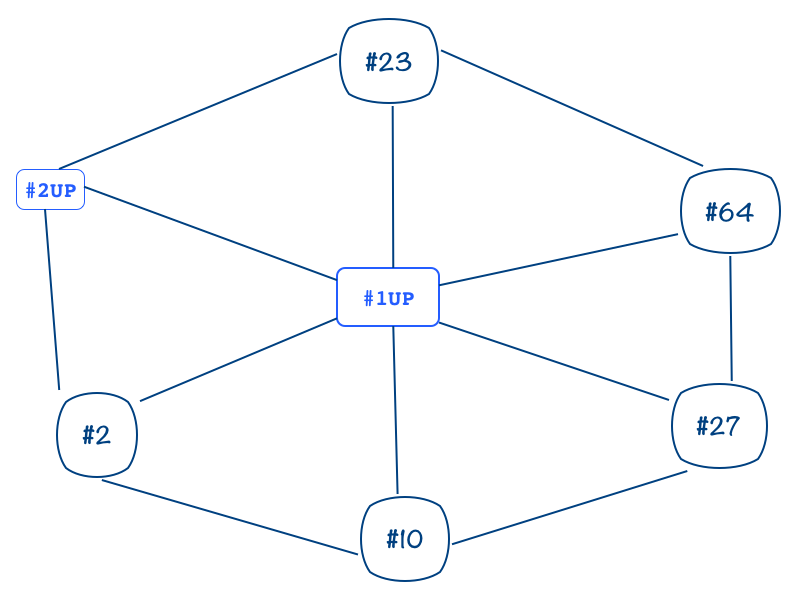
\includegraphics[keepaspectratio=true,scale=0.5]{figuras/grafo.png}
	\caption{Relacionamento entre os elementos da ferramenta.\label{fig05}}
\end{figure}


\section[Desenvolvimento da Proposta]{Desenvolvimento da Proposta}

O gamifier será desenvolvido para plataforma web, onde o usuário irá construir o projeto de gamificação a partir das técnicas de gamificação ou partir das unidades principais, o usuário terá a liberdade de escolher como iniciar o projeto. 

Para desenvolvimento da ferramenta prentende-se fazer uso do SCRUM com adaptações adequadas ao contexto do trabalho, será levantado o backlog de produto, backlog da sprint, escrita de histórias, detalhamento em tarefas e definição de critérios de aceitação, sprints com duração de duas semanas e restrospectiva ao fim das sprints.

\section{Sistema}

O sistema deve ser capaz de importar e exportar os modelos de projetos de gamificação. Apesar de ser um sistema para construção de projetos de gamificações e não um sistema gamificado a inserção de dados e o seu comportamento deve ser leve e fluído, de fácil uso  e interação por parte do usuário. Para não ter os mesmos problemas encontrados na inserção de dados feitos através de planilhas excel e não desmotive o usuário logo no inicio do processo. 

Seria contraditório construir uma ferramenta massante e arcaica dentro de um contexto de gamificação, seria iniciar todo o processo comentendo um erro. O usuário deve se sentir motivado desde o início do uso do sistema até o momento de conclusão do projeto e a usabilidade do sistema terá parte importanta nesse processo. O gamifier deve ser capaz de permitir que o usuário vizualize o projeto como um todo.  A plataforma irá dispor de modelos que servirão de base para a construção dos projetos, caso o usuário sinta necessidade, poderá usar um modelo de gamificação como exemplo. 



\subsection{Requisitos e funcionalidades}
Para desenvolvimendo do sistema foram levantadas histórias de usuário e critérios de aceitação. A



\begin{table}[!htpb]
\centering
\begin{tabular}{|p{1.5cm}|p{12cm}|} \hline

 Número & História de usuário \\ \hline

 1 & Eu, como usuário gostaria de realizar login no sistema, para que eu possa ter acesso aos meus projetos. \\ \hline

 2 & Eu, como usuário gostaria de mudar o status do projeto para público ou privado,  para ter privacidade quando necessário. \\ \hline

 3 & Eu, como usuário gostaria de importar e exportar os projetos de gamificação, para fazer uso em outras plataformas. \\ \hline

 4 & Eu, como usuário, gostaria de finalizar o projeto em um dia diferente do iniciado, para que eu possa modificar o projeto ao longo da construção. \\ \hline

 5 & Eu, como usuário, gostaria de receber um feedback quando o projeto de gamificação não estiver sendo construído de maneira consistente, para que eu possa realizar as modificações necessárias. \\ \hline

 6 & Eu, como usuário, gostaria de construir mais de um projeto, para montar uma galeria de projetos. \\ \hline

 7 & Eu, como usuário, gostaria de reutilizar um projeto finalizado, para aplicar a outro contexto. \\ \hline

 8 & Eu, como usuário, gostaria de escolher a partir de qual elemento inicio o projeto, para ter maior flexibilidade de idéias. \\ \hline

 9 & Eu, como usuário, gostaria de vizualiar uma descrição dos itens que compõem o projeto, para entender o que cada item significa. \\ \hline

 10 & Eu, como usuário, gostaria de vizualizar um tutorial interativo, para entender como funciona a ferramenta. \\ \hline

 11 & Eu, como usuário, gostaria de saber qual tipo de gamifição construi, para entender quais os aspectos serão motivados . \\ \hline

 12 & Eu, como usuário, gostaria de apagar um projeto, para não ter mais acesso ao mesmo. \\ \hline
\end{tabular}
\caption{Histórias de Usuário\label{tab01}
}
\end{table} 





